% ============================================================
%  P1_EquipoNN_Apellido1_Apellido2 / reporte.tex
%  Proyecto de Probabilidad: modelos de lenguaje de n-gramas
%  Compilar con: pdflatex reporte.tex  (dos pasadas)
% ============================================================
\documentclass[11pt,letterpaper]{article}

% ---------- Codificación e idioma ----------
\usepackage[utf8]{inputenc}
\usepackage[T1]{fontenc}
\usepackage[spanish,es-nodecimaldot]{babel} % punto decimal
\usepackage{lmodern}

% ---------- Márgenes: 2.5 cm ----------
\usepackage[letterpaper,margin=2.5cm]{geometry}

% ---------- Interlineado 1.15 ----------
\usepackage{setspace}
\setstretch{1.15}

% ---------- Matemáticas ----------
\usepackage{amsmath,amssymb,amsthm}
\usepackage{mathtools}

% ---------- Figuras y tablas ----------
\usepackage{graphicx}
\usepackage{booktabs}
\usepackage{multirow}
\usepackage{array}
\usepackage{caption}
\captionsetup{font=small,labelfont=bf}
% Tablas: título ARRIBA (caption arriba)
\captionsetup[table]{position=top,skip=4pt}
% Figuras: leyenda ABAJO (caption abajo)
\captionsetup[figure]{position=bottom,skip=4pt}

% ---------- Colores y enlaces ----------
\usepackage{xcolor}
\usepackage[hidelinks]{hyperref}
\usepackage{seqsplit} % Necesario para cortar cadenas largas continuas

% ---------- Código (solo fragmentos <=15 líneas) ----------
\usepackage{listings}
\lstset{
	basicstyle=\ttfamily\small,
	breaklines=true,
	frame=single,
	numbers=left,
	numberstyle=\tiny,
	captionpos=b
}

% ---------- Unidades y números ----------
\usepackage{siunitx}
\sisetup{output-decimal-marker={.}, round-mode=figures, round-precision=4}

% ---------- Encabezado/pie con numeración ----------
\usepackage{fancyhdr}
\pagestyle{fancy}
\fancyhf{}
\fancyhead[L]{\small Proyecto de Probabilidad · Equipo $\langle\text{NN}\rangle$}
\fancyhead[R]{\small \thepage}
\renewcommand{\headrulewidth}{0.4pt}

% ---------- Comandos de apoyo ----------
\newcommand{\BPC}{\mathrm{BPC}}
\newcommand{\PPL}{\mathrm{PPL}}
\newcommand{\KL}{D_{\mathrm{KL}}}
\newcommand{\V}{\mathcal{V}}
\newcommand{\qhat}{\hat{q}}
\newcommand{\phat}{\hat{p}}
\newcommand{\ctx}{h}
\newcommand{\TBD}[1]{\textcolor{red}{[#1]}} % recordatorio visible

% ============================================================
\begin{document}
	
	% ==================== PORTADA ====================
	\begin{titlepage}
		\centering
		\begin{minipage}[c]{0.62\textwidth}
			\centering
			\onehalfspacing
			{\large \textbf{Universidad de Carabobo}} \\
			{\normalsize \textbf{Facultad Experimental de Ciencias y Tecnología}} \\
			{\normalsize \textbf{Departamento de Matematica}} \\
			{\normalsize \textbf{Introducción a la Probabilidad}}
		\end{minipage}
		\par % Fuerza a que lo siguiente vaya debajo y no a la derecha
		
		\vspace*{3cm}
		{\LARGE\bfseries Modelos de lenguaje de n-gramas:\\[4pt]
			predicción del siguiente carácter en español\par}
		\vspace{1.5cm}\par
		\vspace{0.8cm}
		{\large Equipo 03\par}
		\vspace{1cm}
		{\large Integrantes:\par}
		\begin{tabular}{ll}
			Fabian Tovar & C.I. 31456461 \\
			Diego Roche & C.I. 30656951 \\
		\end{tabular}
		\vfill
		{\large Profesor: José Marcano\par}
		\vspace{0.5cm}
		{\large Noviembre de 2026\par}
	\end{titlepage}
	
	% ==================== RESUMEN (<=200 palabras) ====================
	\section*{Resumen}
	\addcontentsline{toc}{section}{Resumen}
	Estimamos modelos de $n$-gramas de caracteres ($n=1,\dots,5$) sobre una traducción al español de \textit{La Divina Comedia} ($668\,786$ caracteres normalizados, $|\mathcal V|=35$). La partición contigua 80/10/10 fija el vocabulario solo con entrenamiento; $\alpha$ se eligió únicamente con validación y el bloque de prueba se evaluó una sola vez. La validación seleccionó $n=5$ con $\alpha=0.03$: BPC de prueba $2.1538$ bits/carácter y perplejidad $4.4499$. Frente a $n=4$, la diferencia fue $\Delta=-0.1518$ bits con intervalo bootstrap del 95\% $[-0.1632,-0.1410]$ (34 bloques, 10 000 remuestras), que excluye el cero. La matriz estocástica del bigrama convergió en 24 iteraciones a una distribución estacionaria que difiere de las frecuencias de unigramas en menos de $10^{-5}$. La desigualdad de Gibbs se cumplió ($KL=0.0016$ bits). La variante opcional con 200 fusiones BPE dio $2.4278$ bits por carácter, peor que el modelo de caracteres. Concluimos que la memoria local de hasta cinco caracteres mejora la predicción sin sobreajuste apreciable, aunque el modelo no capta semántica ni dependencias largas.
	
	% ==================== 1. INTRODUCCIÓN ====================
	\section{Introducción}
	Este trabajo aplica la sección S01 ''El lenguaje como distribución de probabilidad'' del libro "Modelos de Lenguaje de Gran Escala" (Dr. José G. Marcano). Predecir el siguiente carácter de un texto es el ejemplo más directo de un modelo de lenguaje: la probabilidad de una cadena se factoriza, por la regla de la cadena (Prop. 1.1.3), en el producto de condicionales de cada símbolo dado su contexto inmediato. Si el contexto se limita a los $n-1$ caracteres anteriores obtenemos una cadena de Markov de orden $n-1$ (Def. 1.1.6). El proyecto pregunta cuál de esos órdenes predice mejor un texto español real, cómo debe suavizarse y cuánta incertidumbre tiene la comparación.
	
	El corpus se normalizó y dividió en bloques contiguos 80/10/10; el par $(n,\alpha)$ se fijó con validación y la prueba se evaluó al final. Las secciones 2--6 cubren marco, datos, métodos, resultados y verificaciones; la 7 responde al enunciado y la 8 concluye.
	
	% ==================== 2. MARCO PROBABILÍSTICO ====================
	\section{Marco probabilístico}
	
	Sea $\mathcal V$ el alfabeto finito de símbolos (Def. 1.1.1); aquí $|\mathcal V|=35$. Escribimos $x_{1:T}$ para una cadena de caracteres y $h_t=x_{t-n+1:t-1}$ para su contexto de longitud $n-1$. La regla de la cadena y la hipótesis de Markov dan
	

	\begin{equation}
		q(x_{1:T})=\prod_{t=1}^{T}q(x_t\mid x_{1:t-1})
		\;\approx\;\prod_{t=1}^{T}q(x_t\mid x_{t-n+1:t-1}). \tag{1}
	\end{equation}
	
	El signo $\approx$ indica la hipótesis de Markov: se sustituye el contexto completo $x_{1:t-1}$ de la regla de la cadena por sus $n-1$ caracteres finales; para $n=1$ la igualdad es exacta.
	
	La estimación por máxima verosimilitud (Prop. 1.1.8) es la frecuencia relativa
	
	\begin{equation}
		\hat q(y\mid h)=\frac{c(h,y)}{c(h)},\qquad c(h)=\sum_{y\in\mathcal V}c(h,y),
	\end{equation}
	
	donde $c(h,y)$ cuenta las veces que $y$ sigue al contexto $h$ en entrenamiento. Si el par no aparece, la MLE asigna probabilidad cero. El suavizado aditivo (Prop. 1.1.14) evita los ceros sumando un seudocuento $\alpha>0$ a cada par; $\alpha$ controla cuánta masa se reparte entre símbolos no vistos:
	
	\begin{equation}
		\hat q_\alpha(y\mid h)=\frac{c(h,y)+\alpha}{c(h)+\alpha|\mathcal V|},
		\qquad \alpha=0 \text{ es la MLE}. \tag{2}
	\end{equation}
	
	La entropía satisface $H(p)=-\sum_i p_i\log_2 p_i\le\log_2|\mathcal V|$, con igualdad solo bajo uniformidad (Prop. 1.1.15). En modelado de caracteres se reporta

	\begin{equation}
		\mathrm{BPC}=-\frac{1}{N_e}\sum_{t=1}^{N_e}\log_2\hat q_\alpha(x_t\mid h_t),
		\qquad \mathrm{PPL}=2^{\mathrm{BPC}}, \tag{3}
	\end{equation}
	
	donde $N_e$ es el número de caracteres evaluados (Def. 1.1.20). El BPC es la entropía cruzada empírica y $\mathrm{PPL}=2^{\mathrm{BPC}}$. La entropía cruzada $H(p,q)$ mide el costo medio de codificar con $q$ datos de $p$; por la desigualdad de Gibbs (Teo. 1.1.27), $H(p,q)-H(p)=D_{\mathrm{KL}}(p\|q)\ge0$ (Def. 1.1.17):
	\begin{equation}
		H(p)=-\sum_i p_i\log_2 p_i\le H(p,q)=-\sum_i p_i\log_2 q_i,
		\qquad D_{\mathrm{KL}}(p\|q)=H(p,q)-H(p). \tag{4}
	\end{equation}
	Para una matriz de transición positiva $P$, la entrada $P_{yz}$ es la probabilidad de pasar del símbolo $y$ al símbolo $z$, y $\pi_y$ es la probabilidad de estar en $y$ en régimen estacionario; entonces $\pi P=\pi$ y $\pi_0P^t\to\pi$ (Teo. 1.1.40). Se itera hasta $\|\pi_t-\pi_{t-1}\|_1<10^{-10}$. Finalmente, el bootstrap (Def. 1.1.44) remuestrea con reemplazo unidades consideradas independientes; aquí son bloques contiguos de prueba, no caracteres, por la dependencia local de la cadena.
	
	% ==================== 3. DATOS ====================
	\section{Datos}	

	\subsection{Fuente y normalización}
	La fuente es ''La Divina Comedia'', Dante Alighieri, traducción de Manuel Aranda y Sanjuán (Barcelona, 1871), descargada de `https://archive.org/details/ladivinacomedia57303gut` el 21 de noviembre de 2026. Es texto plano en CP1252, copia del Gutenberg eBook \#57303; la traducción del siglo XIX es de dominio público y la procedencia está registrada en `datos/FUENTE.md`. El script `preparar.py` recorta el poema, elimina encabezados, ilustraciones y notas, pasa a minúsculas, colapsa espacios y saltos repetidos y sustituye por `\#` todo carácter fuera del alfabeto permitido: letras minúsculas `a`--`z`, vocales acentuadas `áéíóú`, `ñ`, `ü`, espacio y el propio `\#`. El vocabulario $\mathcal V$ se fija solo con entrenamiento.

	\subsection{Participación}
	% ---- T1 ----
	\begin{table}[htbp]
		\centering
		\caption{T1. Tamaño de cada partición y $|\V|$.}
		\label{tab:T1}
		\begin{tabular}{lrr}
			\toprule
			Partición & Caracteres & \% \\
			\midrule
			Entrenamiento & {535\,028} & 80 \\
			Validación    & {66\,879} & 10 \\
			Prueba        & {66\,879} & 10 \\
			\midrule
			$|\V|$        & {668\,786} & \\
			\bottomrule
		\end{tabular}
	\end{table}
	
	% ---- F1 ----
	\begin{figure}[htbp]
		\centering
		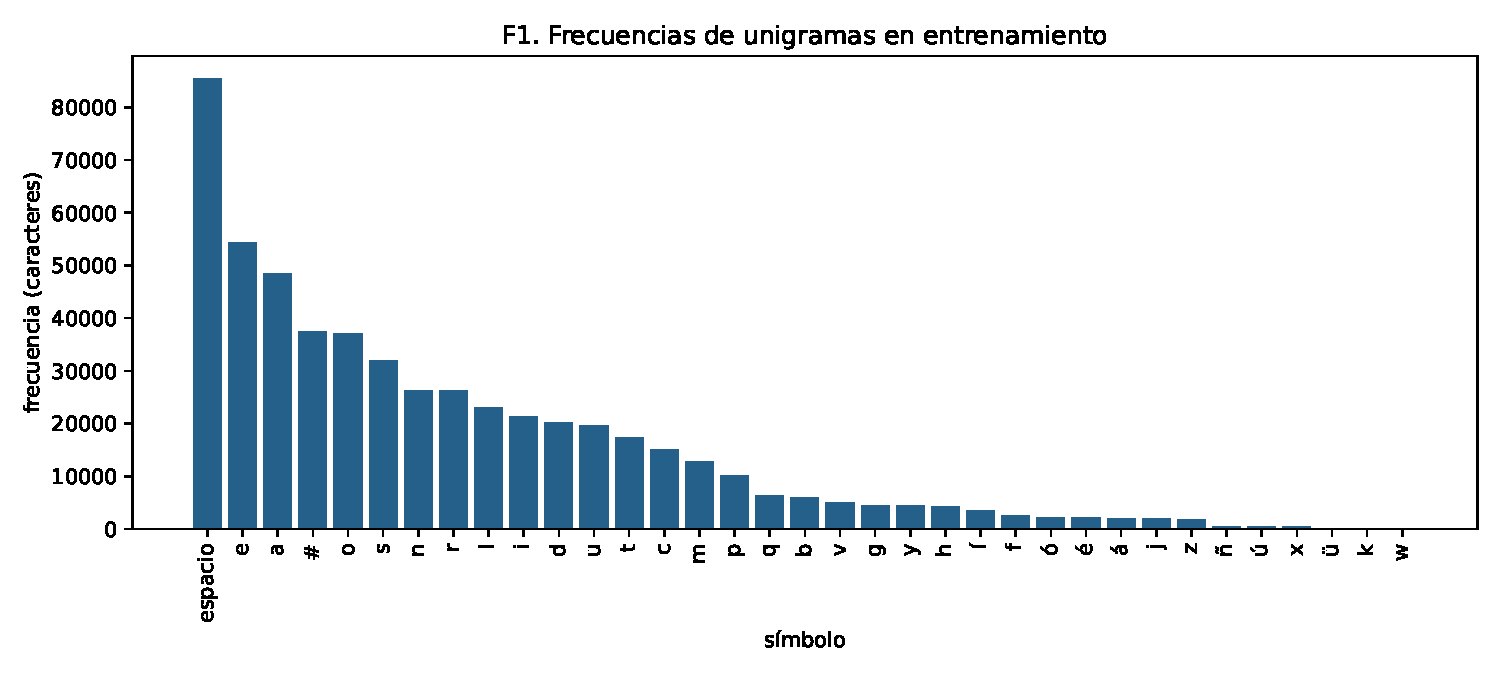
\includegraphics[width=0.8\textwidth]{resultados/F1.pdf} %F1_frecuencias
		\caption{F1. Frecuencias de los símbolos de $\V$, ordenadas de mayor a menor.}
		\label{fig:F1}
	\end{figure}
	\vspace{0.5cm}
	% ==================== 4. MÉTODOS ====================
	\section{Métodos}
	Esta sección describe el flujo que transforma el corpus de la Sección~3 en los resultados de la Sección~5. El orden de ejecución es \texttt{preparar.py} $\rightarrow$ \texttt{pruebas.py} $\rightarrow$ \texttt{experimentos.py A/B}: el primero escribe las particiones y \texttt{resultados/vocabulario.json}; el segundo verifica la API; el tercero lee los datos con \texttt{cargar\_datos()} y genera tablas y figuras (en PDF y PNG). \texttt{modelos.py} centraliza los conteos, probabilidades, secuencias, BPC y PPL para las seis fases, mientras que las fases de A (2, 4 y 6) y de B (3, 5 y 7) comparten \texttt{calcular\_alpha\_por\_n}, asegurando que el suavizado seleccionado en validación alimente todas las mediciones.
	
	\subsection{Conteos y MLE}
	La función \texttt{ModeloNgramas.\_ajustar} recorre \texttt{train} desde $k=n-1$ acumulando las frecuencias del contexto $c(h)$ (donde $h=x_{t-k:t-1}$) y del par $c(h,y)$. Al almacenar solo pares observados, en T2 los contextos pasan de 1 ($n=1$) a $23\,672$ ($n=5$) y los pares de 35 a $66\,833$ (\texttt{len(modelo.contextos)} y suma de \texttt{modelo.pares}). La estimación de máxima verosimilitud (MLE) es
	\begin{equation}
		\hat q_0(y\mid h)=\frac{c(h,y)}{c(h)},\qquad \hat q_0(y\mid h)=0\ \text{si}\ c(h,y)=0.
		\label{eq:mle}
	\end{equation}
	Mediante \texttt{suma\_condicionales(h)} se verifica que cada distribución suma 1 dentro de una tolerancia de $10^{-12}$ (error máximo de $0$ para $n=1,2$ y $1.110\times10^{-16}$ para $n=3,4,5$ en \texttt{max\_error\_sumas}).
	
	Para evaluar todos los caracteres de validación ($66\,879$) y prueba sin descartar posiciones iniciales, \texttt{prefijo\_de(train, n)} y \texttt{secuencias(val, prefijo)} anteponen los últimos $n-1$ caracteres de \texttt{train} (o de \texttt{val + test[:inicio]} en prueba); en entrenamiento (Fase~4) no se usa prefijo, evaluando $N_e=535\,028-(n-1)$ caracteres. En validación, la fracción de caracteres no vistos ($\hat q_0=0$) crece de $0$ ($n=1$) a $0.039100$ ($n=5$, $2\,615$ caracteres), lo que haría diverger el BPC de la MLE. Sobre entrenamiento, la log-verosimilitud en base 2 (\texttt{log2\_verosimilitud\_train} de T2) se calcula sobre pares observados como
	\begin{equation}
		\ell_0=\sum_{h}\sum_{y:\,c(h,y)>0} c(h,y)\,\log_2\frac{c(h,y)}{c(h)}.
		\label{eq:loglik0}
	\end{equation}
	Para verificar la Prop.~1.1.8, \texttt{\_elegir\_perturbaciones} selecciona el contexto más frecuente, su símbolo más probable $y_o$ y dos destinos $y_d$, transfiriendo $\delta=0.01$ de masa ($\hat q_1(y_o\mid h)=q_o-\delta$, $\hat q_1(y_d\mid h)=q_d+\delta$). La verosimilitud perturbada,
	\begin{equation}
		\ell_1=\ell_0+c(h,y_o)\log_2\frac{q_o-\delta}{q_o}
		+c(h,y_d)\log_2\frac{q_d+\delta}{q_d},
		\label{eq:loglik1}
	\end{equation}
	satisface $\ell_0>\ell_1$ en todos los órdenes (tolerancia $10^{-9}$), registrando los símbolos en T2 (escapando \texttt{\#} como \texttt{\textbackslash\#}).
	
	\subsection{Suavizado y selección de $\alpha$}
	Para evitar probabilidades nulas, se aplica suavizado con $\alpha>0$ (Ec.~(2)) evaluando los 35 pares por contexto. Se entrenan $5\times7=35$ modelos combinando $n\in\{1,\dots,5\}$ y $\alpha\in\{0.001,0.003,0.01,0.03,0.1,0.3,1\}$ sobre \texttt{train}, midiendo en validación con prefijo de entrenamiento:
	\begin{equation}
		\mathrm{BPC}_{\mathrm{val}}(n,\alpha)
		=-\frac{1}{66\,879}\sum_{t=1}^{66\,879}\log_2\hat q_\alpha(x_t\mid h_t).
		\label{eq:bpc_val}
	\end{equation}
	La función \texttt{bpc\_validacion\_por\_alpha} ignora explícitamente \texttt{\_test}. Para cada $n$, \texttt{asegurar\_alpha\_por\_n} elige el mínimo BPC desempatando por menor $\alpha$ (\texttt{min(ALPHAS, key=lambda a: (bpc[a], a))}) y guarda la caché en \texttt{resultados/alpha\_por\_n.json} (verificada en la Fase~3). Los resultados se escriben en \texttt{validacion\_alpha.csv} (marcados con \texttt{es\_mejor}) y se grafican en F2. La selección óptima es $\alpha=\{1:1,\ 2:0.03,\ 3:0.1,\ 4:0.03,\ 5:0.03\}$ (recogida en T5), evitando diluir masa en órdenes altos.
	
	\subsection{Métricas}
	Con los $\alpha$ óptimos, \texttt{bpc\_validacion\_por\_n} y \texttt{mejor\_n\_por\_validacion} seleccionan el orden óptimo $n^\star=5$ ($2.183777$ bits/carácter) antes de acceder a prueba. Posteriormente, \texttt{evaluar\_prueba\_una\_vez} verifica la ausencia de \texttt{resultados/metricas\_prueba.csv} (salvo con \texttt{--forzar-prueba}) para garantizar una única evaluación: divide los $66\,879$ caracteres de prueba en 34 bloques contiguos (33 de $2\,000$ y uno de $879$) con prefijo \texttt{val + test[:inicio]}, guarda el BPC por bloque y dibuja el promedio acumulado en F4 para $n^\star$.
	
	El BPC global de prueba es el promedio ponderado por longitud de bloque $\ell_j$, con perplejidad $\mathrm{PPL}=2^{\mathrm{BPC}_{\mathrm{prueba}}}$ (Ec.~(3)):
	\begin{equation}
		\mathrm{BPC}_{\mathrm{prueba}}(n)
		=\frac{\sum_j \mathrm{BPC}_j(n)\,\ell_j}{\sum_j \ell_j}.
		\label{eq:bpc_test}
	\end{equation}
	Junto con \texttt{.bpc(train)}, el BPC de validación y \texttt{es\_mejor\_n}, se conforma \texttt{T3.csv} y la figura F3; para $n^\star=5$, se obtiene un BPC de entrenamiento de $1.848241$ y de prueba de $2.153786$ ($\mathrm{PPL}=4.4499$). Asimismo, se verifica la desigualdad de Gibbs (Ec.~(4)) entre la distribución empírica $p$ de prueba y el unigrama suavizado $q$ ($\alpha=1$), comprobando $D_{\mathrm{KL}}(p\|q)=4.192472-4.190885=0.001587\ge-10^{-12}$ bits en T4.
	
	\subsection{Simulación de la cadena}
	A partir del bigrama suavizado ($\alpha=0.03$), se construye la matriz de transición $P_{yz}=\hat q_\alpha(z\mid y)$ sobre los 35 símbolos, verificando en \texttt{verificacion\_simulacion.csv} que cada fila suma 1 (error máximo $3.331\times10^{-16}$) y que toda entrada es positiva (mínimo $3.509\times10^{-7}$). Partiendo de $\pi_0=(1/35,\dots,1/35)$, la iteración $\pi_{t+1}=\pi_t P$ converge en 24 pasos ($\|\pi_{t+1}-\pi_t\|_1=5.610\times10^{-11}<10^{-10}$) a la distribución estacionaria $\pi$, cuya diferencia máxima respecto a las frecuencias empíricas $c(y)/535\,028$ es menor que $10^{-5}$ (\texttt{estacionaria.csv} y F5).
	
	Para muestrear, \texttt{numpy.random.default\_rng(20261123)} genera tres secuencias de 300 caracteres para $n=2,3,5$ partiendo del contexto \texttt{" que "} (verificado en \texttt{train}), eligiendo cada símbolo con \texttt{rng.choice} y desplazando la ventana de tamaño $n-1$. Las muestras se guardan en \texttt{muestras\_simulacion.csv} y se transcriben en el Anexo~C.
	
	\subsection{Bootstrap por bloques}
	Sin reevaluar prueba, se leen las métricas de la Fase~4 mediante \texttt{leer\_metricas\_prueba()} y se comparan los modelos $n^\star=5$ y $n^\star-1=4$ bloque a bloque:
	\begin{equation}
		\Delta_j=\mathrm{BPC}_j(5)-\mathrm{BPC}_j(4),
		\label{eq:delta_j}
	\end{equation}
	cuya media no ponderada en los 34 bloques es $-0.151797$ bits/carácter (frente a $-0.151152$ ponderado por caracteres en T4). Para respetar la dependencia local, \texttt{numpy.random.default\_rng(20261122)} extrae $10\,000$ remuestras bootstrap de los 34 bloques con reemplazo, obteniendo el intervalo de confianza del 95\,\% mediante percentiles:
	\begin{equation}
		\mathrm{IC}_{95\%}=
		\big[Q_{0.025}(\bar\Delta^*),\ Q_{0.975}(\bar\Delta^*)\big]
		=[-0.163172,\ -0.140998],
		\label{eq:ic95}
	\end{equation}
	con marca \texttt{intervalo\_excluye\_cero} igual a 1.
	
	\subsection{Tokenización BPE (Fase 7 opcional)}
	\texttt{\_aprender\_bpe} ejecuta 200 iteraciones sobre \texttt{train} contando pares adyacentes con \texttt{Counter} y fusionando el más frecuente (desempatando por primera aparición). Luego, \texttt{\_tokenizar} aplica las 200 reglas a \texttt{train}, \texttt{val} y \texttt{test}, generando un vocabulario de $1\,900$ tokens (107 exclusivos de validación/prueba) mapeados a caracteres únicos (\texttt{chr(i+1)}) para reutilizar \texttt{ModeloNgramas}.
	
	Se ajusta un bigrama de tokens seleccionando $\alpha=0.03$ en validación tras escalar a bits por carácter:
	\begin{equation}
		\mathrm{BPC}_{\text{carácter}}^{\text{BPE}}
		=\mathrm{BPC}_{\text{token}}\,
		\frac{N_{\text{tokens}}}{N_{\text{caracteres}}}.
		\label{eq:bpe_bpc}
	\end{equation}
	Al evaluar prueba una única vez (factor $26\,178/66\,879$), se obtiene $2.427847$ bits/carácter, superando en $+0.274061$ al modelo de caracteres de referencia de \texttt{T3.csv} ($2.153786$). Los resultados y la marca \texttt{metricas\_prueba\_csv\_reescrito=0} se registran en \texttt{bpe\_resultados.csv}.	\section{Resultados}
		
	\subsection{Contextos y ceros (Fase 2)}
	% ---- T2 ----
\begin{table}[htbp]
	\centering
	\caption{Conteos, ceros en validación y log-verosimilitud de la MLE.}
	\label{tab:T2}
	\resizebox{\textwidth}{!}{%
		\begin{tabular}{r r r r r r r}
			\toprule
			$n$ & Contextos & Pares obs. & Fracc. ceros (val.) & $\log_2$ verosim. MLE & $\log_2$ pert. 1 & $\log_2$ pert. 2 \\
			\midrule
			1 & $1$      & $35$     & $0.000000$ & $-2\,246\,683.4227$ & $-2\,247\,291.6974$ & $-2\,247\,332.9410$ \\
			2 & $35$     & $656$    & $0.000030$ & $-1\,740\,981.3494$ & $-1\,741\,104.1434$ & $-1\,741\,110.6891$ \\
			3 & $656$    & $5\,398$ & $0.001824$ & $-1\,452\,309.3304$ & $-1\,452\,329.6431$ & $-1\,452\,334.2530$ \\
			4 & $5\,398$ & $23\,672$& $0.011199$ & $-1\,186\,858.9667$ & $-1\,186\,867.6063$ & $-1\,186\,876.2864$ \\
			5 & $23\,672$& $66\,833$& $0.039100$ & $-960\,983.0723$   & $-960\,988.8387$   & $-960\,994.4501$   \\
			\bottomrule
		\end{tabular}%
	}
\end{table} 
	\paragraph{Procedencia de las cifras.}
	Cada fila de T2 la escribe \texttt{fase2\_mle} con un modelo MLE distinto, uno por orden. Las columnas \texttt{contextos\_observados} y \texttt{pares\_observados} salen de los contadores descritos en \S 4.1; \texttt{max\_error\_sumas} es el mayor $|1 - \sum_y \hat q_0(y \mid h)|$; \texttt{fraccion\_ceros\_validacion} es \texttt{ceros\_validacion / caracteres\_validacion}, con $66\,879$ caracteres evaluados en los cinco órdenes; y las tres log-verosimilitudes se calculan con las Ecs.~(6) y (7) y se redondean a cuatro decimales al escribir el CSV. Las columnas finales registran el contexto y los símbolos efectivamente perturbados, de modo que cada comparación es reproducible. Las condicionales suman 1 con error máximo $1.110 \times 10^{-16}$; la MLE supera a las dos perturbaciones en los cinco órdenes (Prop.~1.1.8) y los ceros de validación crecen de $0$ a $0.0391$, como predice la rarefacción de los contextos.
	
	\subsection{Suavizado y elección de $\alpha$ (Fase 3)}
	% ---- F2 ----
	\begin{figure}[htbp]
		\centering
		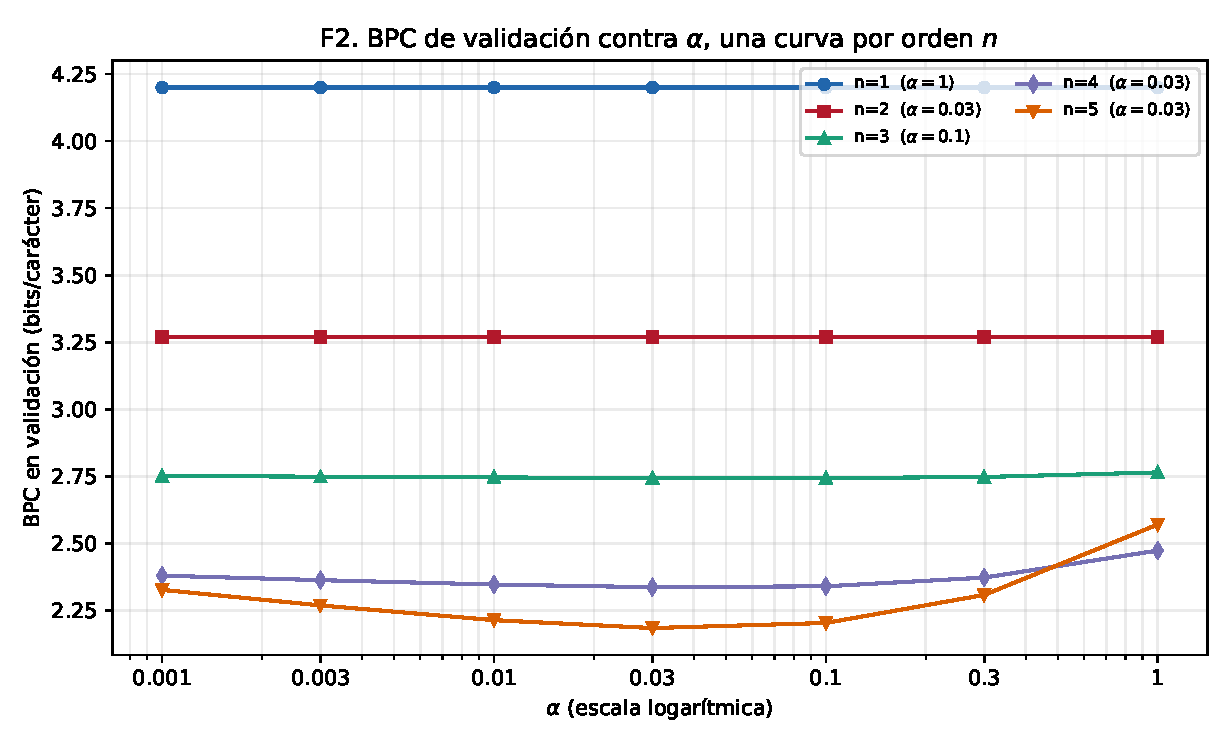
\includegraphics[width=0.8\textwidth]{resultados/F2.pdf} %F2_bpc_vs_alpha
		\caption{F2. BPC de validación contra $\alpha$ (eje horizontal logarítmico), una curva por $n$.}
		\label{fig:F2}
	\end{figure}
	La tabla T3 recoge el mínimo de cada curva.
	
	\begin{table}[htbp]
		\centering
		\caption{$\alpha$ seleccionado por validación y BPC de validación resultante.}
		\label{tab:T5}
		\begin{tabular}{r r r}
			\toprule
			$n$ & $\alpha$ elegido & BPC de validación (bits/carácter) \\
			\midrule
			1 & 1    & 4.199982 \\
			2 & 0.03 & 3.268909 \\
			3 & 0.1  & 2.743152 \\
			4 & 0.03 & 2.336153 \\
			5 & 0.03 & 2.183777 \\
			\bottomrule
		\end{tabular}
	\end{table}
	
	\paragraph{Procedencia de las cifras.}
	F2 la dibuja \texttt{fase3\_alpha} directamente desde la matriz \texttt{bpc\_validacion\_por\_alpha} (35 ajustes, todos con \texttt{train} y \texttt{val}); T5 no es una tabla nueva: es el mínimo de cada una de las cinco curvas, es decir la intersección de \texttt{validacion\_alpha.csv} con \texttt{alpha\_por\_n.json}. Los BPC de validación se escriben con diez decimales en el CSV y con seis en T4, de modo que las cifras del informe coinciden con la precisión declarada en cada tabla. La elección no es monótona en $n$; la explicación está en \S 7.3 y el protocolo de selección en \S 4.2.
	
	\subsection{Evaluación en prueba (Fase 4)}
	\begin{table}[htbp]
		\centering
		\caption{Resultados de entrenamiento, validación y prueba por orden $n$.}
		\label{tab:T3}
		\begin{tabular}{r r r r r r}
			\toprule
			$n$ & $\alpha$ & BPC val. & BPC train & BPC prueba & PPL prueba \\
			\midrule
			1 & 1    & 4.199982 & 4.199190 & 4.192472 & 18.2835 \\
			2 & 0.03 & 3.268909 & 3.254051 & 3.257788 & 9.5652  \\
			3 & 0.1  & 2.743152 & 2.718575 & 2.718914 & 6.5838  \\
			4 & 0.03 & 2.336153 & 2.230232 & 2.304938 & 4.9415  \\
			5 & 0.03 & 2.183777 & 1.848241 & 2.153786 & 4.4499  \\
			\bottomrule
		\end{tabular}
	\end{table}
	
	La figura F3 compara la evolución del BPC de entrenamiento y de prueba con el orden $n$.
	
	% ---- F3 ----
	\begin{figure}[htbp]
		\centering
		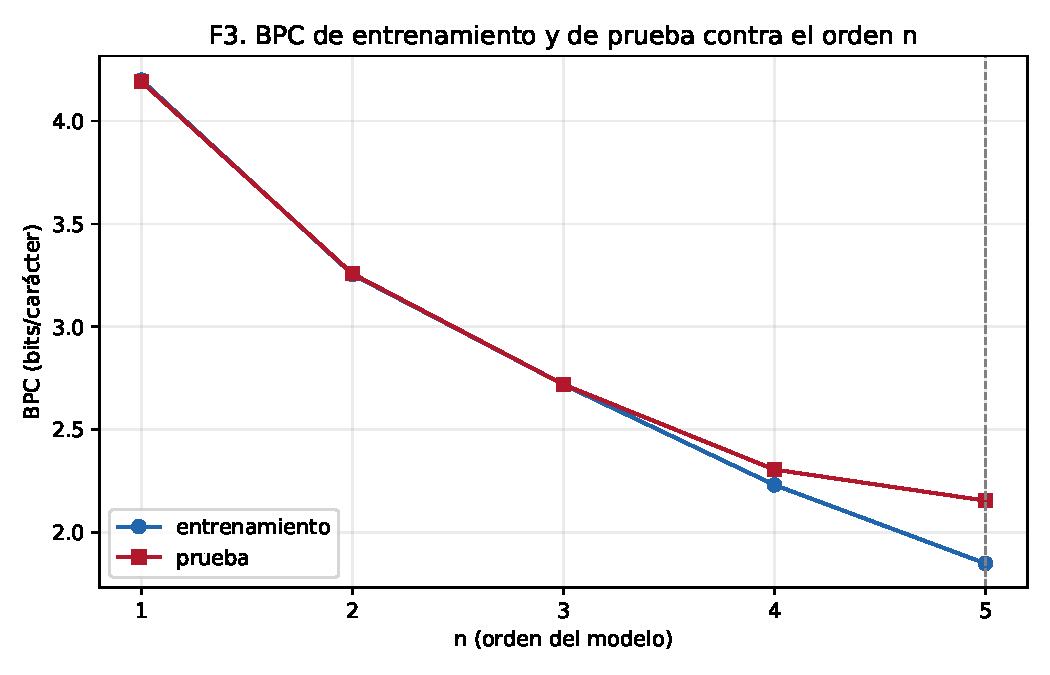
\includegraphics[width=0.8\textwidth]{resultados/F3.pdf} %F3_bpc_vs_n
		\caption{F3. BPC de entrenamiento y de prueba contra $n$ en la misma gráfica.}
		\label{fig:F3}
	\end{figure}
	La figura F4 muestra cómo se estabiliza el promedio acumulado de pérdida dentro del bloque de prueba.
	% ---- F4 ----
	\begin{figure}[htbp]
		\centering
		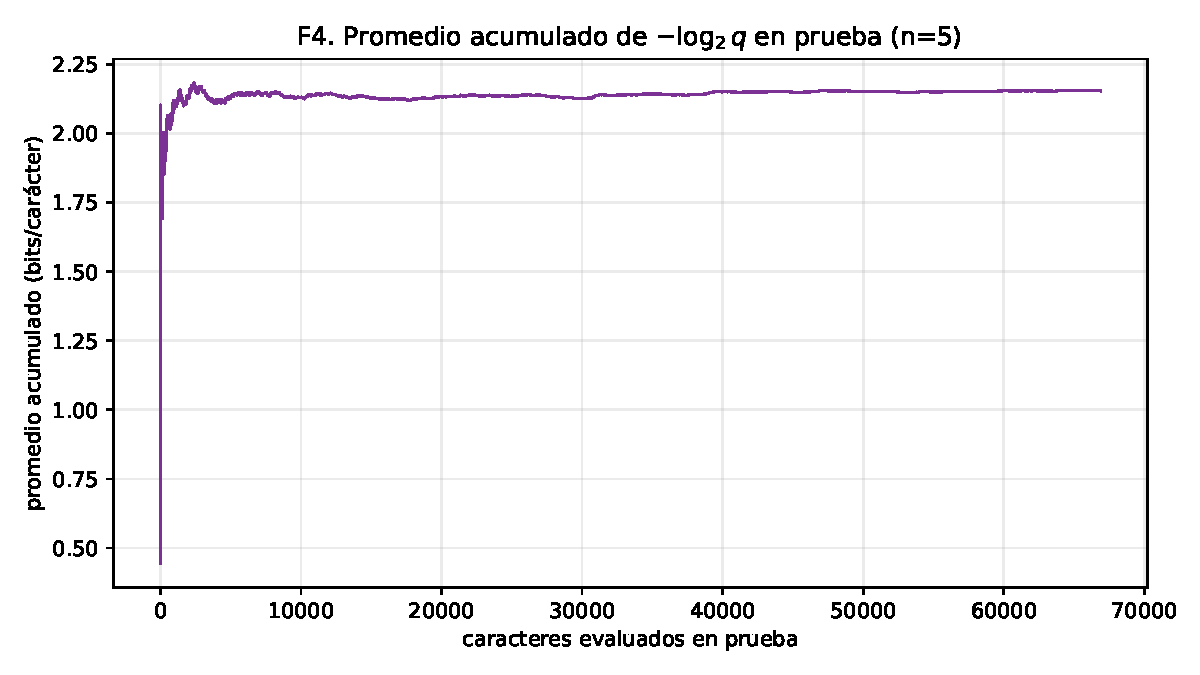
\includegraphics[width=0.8\textwidth]{resultados/F4.pdf} %F4_promedio_acumulado
		\caption{F4. Promedio acumulado de $-\log_2 \qhat$ a lo largo del texto de prueba.}
		\label{fig:F4}
	\end{figure}
	\paragraph{Procedencia de las cifras.}
	Las cinco filas de T4 las produce \texttt{fase4\_evaluacion} con \texttt{alpha\_por\_n.json}, los BPC de validación ya calculados, \texttt{.bpc(train)} y el promedio ponderado de los bloques de \texttt{metricas\_prueba.csv} descrito en la Ec.~(9). La PPL se obtiene como $2^{\mathrm{BPC}_{\mathrm{prueba}}}$. Las columnas \texttt{H\_p\_prueba}, \texttt{H\_pq\_prueba} y \texttt{KL\_prueba} se repiten iguales en todas las filas porque son una sola verificación global, calculada con el unigrama y las frecuencias de prueba. F3 se dibuja en la misma función a partir de \texttt{bpc\_train} y \texttt{bpc\_test}; F4 se genera dentro de \texttt{evaluar\_prueba\_una\_vez} en la única evaluación de prueba. La prueba confirma el orden elegido: BPC mínimo $2.1538$ bits y $\mathrm{KL} = 0.001587$ bits para el unigrama ($4.190885 \le 4.192472$).
	

	\subsection{Simulación y distribución estacionaria (Fase 5)}
	La figura F5 compara la distribución estacionaria del bigrama con las frecuencias observadas.
	
	% ---- F5 ----
	\begin{figure}[htbp]
		\centering
		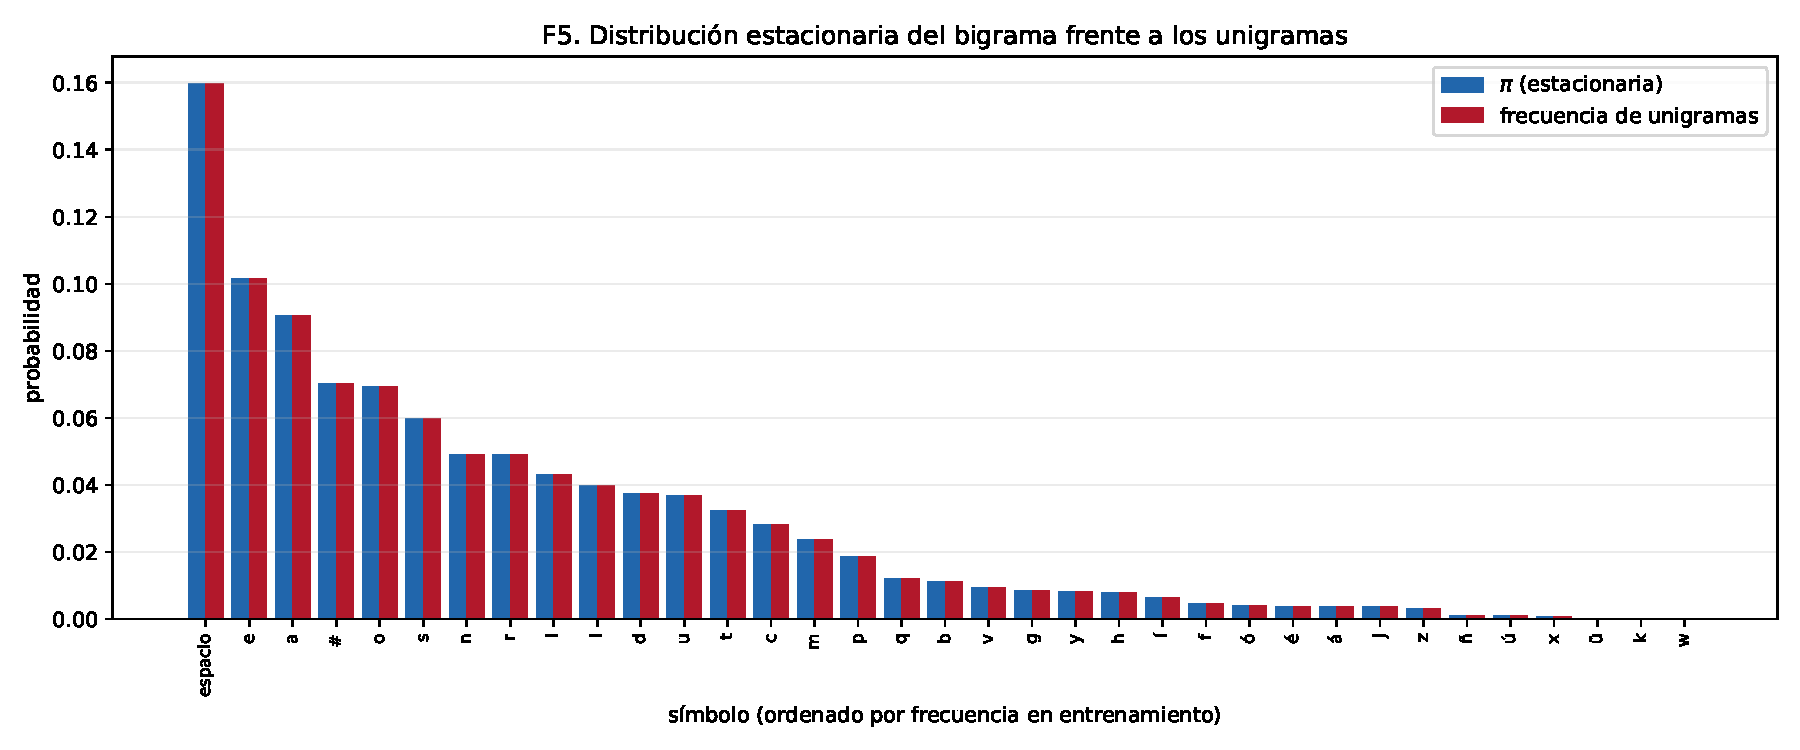
\includegraphics[width=0.8\textwidth]{resultados/F5.pdf} %F5_pi_vs_unigramas
		\caption{F5. Distribución estacionaria $\pi$ frente a las frecuencias de unigramas.}
		\label{fig:F5}
	\end{figure}

	La tabla T5 resume la convergencia y la simulación.
	
	\begin{table}[htbp]
		\centering
		\caption{Verificación de la simulación.}
		\label{tab:T6}
		\begin{tabular}{l l}
			\toprule
			Magnitud & Valor \\
			\midrule
			Tamaño de $P$ & $35 \times 35$ \\
			Error máximo de sumas por fila & $3.331 \times 10^{-16}$ \\
			Entrada mínima de $P$ & $3.509 \times 10^{-7}$ \\
			Iteraciones de potencias & 24 \\
			$\|\pi_t - \pi_{t-1}\|_1$ final & $5.610 \times 10^{-11}$ \\
			$\max_y |\pi_y - \hat p(y)|$ & $< 10^{-5}$ \\
			Semilla / longitud de muestra & 20261123 / 300 caracteres \\
			\bottomrule
		\end{tabular}
	\end{table}
	
	\paragraph{Procedencia de las cifras.}
	Los 35 pares que se comparan en F5 están en \texttt{estacionaria.csv}, con columnas $\pi$, frecuencia de entrenamiento y diferencia; T6 resume los escalares que \texttt{fase5\_simulacion} escribe en \texttt{verificacion\_simulacion.csv} porque son comprobaciones, no resultados de predicción. Las tres cadenas generadas se guardan en \texttt{muestras\_simulacion.csv} con su orden, su $\alpha$, la semilla y el contexto inicial, y se transcriben sin cambios en el Anexo~C. Los símbolos más probables son espacio ($0.1598$), $e$ ($0.1017$), $a$ ($0.0905$) y \texttt{\#} ($0.0702$), en el mismo orden que en entrenamiento; la diferencia máxima entre $\pi$ y la frecuencia empírica es menor que $10^{-5}$.
	
	\subsection{Incertidumbre (Fase 6)}
	\begin{table}[htbp]
		\centering
		\caption{Bootstrap por bloques de $\Delta = \mathrm{BPC}(n^\star) - \mathrm{BPC}(n^\star - 1)$.}
		\label{tab:T4}
		\begin{tabular}{l l}
			\toprule
			Magnitud & Valor \\
			\midrule
			Mejor orden $n^\star$ / orden comparado & 5 / 4 \\
			Número de bloques & 34 \\
			Tamaño de bloque & 2000 caracteres \\
			Media de $\Delta_j$ & $-0.151797$ bits/carácter \\
			IC 95\,\% (percentil) & $[-0.163172,\, -0.140998]$ bits/carácter \\
			Remuestras / semilla & 10\,000 / 20261122 \\
			\bottomrule
		\end{tabular}
	\end{table}
	
	\paragraph{Procedencia de las cifras.}
	T6 la escribe \texttt{fase6\_bootstrap} a partir de \texttt{leer\_metricas\_prueba()}: toma las columnas \texttt{bpc} de los órdenes 5 y 4, forma las 34 diferencias de la Ec.~(10), las remuestrea con la semilla \texttt{20261122} y guarda la media, los percentiles y la marca \texttt{intervalo\_excluye\_cero}. El IC excluye el cero. T4 da la diferencia global sobre toda la prueba, $2.153786 - 2.304938 = -0.151152$ bits, mientras T6 da la media no ponderada de las 34 diferencias por bloque, $-0.151797$ bits. No coinciden exactamente porque T4 divide por los $66\,879$ caracteres del bloque completo y T6 pesa cada bloque por igual, incluido el último de $879$ caracteres; son dos estimadores del mismo efecto, no una contradicción.
	
	\subsection{Tokenización BPE (Fase 7)}
	
	La tabla T7 compara el bigrama de tokens con el modelo de caracteres usando caracteres como denominador común.
	
	\begin{table}[htbp]
		\centering
		\caption{Resultado de la Fase 7 y comparación justa por carácter.}
		\label{tab:T7}
		\begin{tabular}{l l}
			\toprule
			Magnitud & Valor \\
			\midrule
			Fusiones BPE & 200 \\
			$|\mathcal{V}_{\text{tokens}}|$ & 1900 \\
			Tokens nuevos en validación/prueba & 107 \\
			$\alpha$ elegido en validación & 0.03 \\
			Tokens de entrenamiento / prueba & 209\,817 / 26\,178 \\
			Caracteres de prueba & $66\,879$ \\
			BPC por carácter (BPE) & 2.427847 \\
			BPC por carácter (Fase 4, $n=5$) & 2.153786 \\
			Diferencia BPE $-$ Fase 4 & $+0.274061$ \\
			\bottomrule
		\end{tabular}
	\end{table}
	
	\paragraph{Procedencia de las cifras.}
	Todas las entradas de T7 provienen de \texttt{bpe\_resultados.csv}, escrito por \texttt{fase7\_bpe}: el número de fusiones y de tokens se cuenta durante la codificación, el $\alpha$ se selecciona en validación con la Ec.~(12) y el BPC de prueba se mide con prefijo de validación. El BPC de referencia se lee de \texttt{T3.csv} (fila marcada \texttt{es\_mejor\_n=1}) y la última fila del CSV confirma que \texttt{metricas\_prueba.csv} no se reescribió. Los 107 tokens nuevos solo permiten codificar validación y prueba; no aportan conteos al ajuste. Con el mismo denominador, BPE queda $0.2741$ bits/carácter por encima de $n=5$: las 200 fusiones reducen la secuencia a $209\,817$ tokens, pero reparten las estimaciones entre $1900$ símbolos en lugar de $35$.
	
	
	% ==================== 6. VERIFICACIONES ====================
	\section{Verificaciones}
	\paragraph{Cómo se ejecutaron.}
	Hay dos grupos de comprobaciones. El primero corresponde a \texttt{python codigo/pruebas.py}: la función \texttt{prueba\_abracadabra} contrasta los seis números de la tabla~2 del enunciado usando directamente la API de \texttt{modelos.py}; \texttt{prueba\_gibbs} comprueba la Ec.~(4) con una distribución $2 \times 2$; y \texttt{prueba\_estacionaria} itera una matriz conocida hasta recobrar $(2/3,\, 1/3)$. El segundo grupo está repartido en las fases: \texttt{fase2\_mle} verifica las sumas condicionales, \texttt{fase4\_evaluacion} verifica Gibbs sobre la prueba, \texttt{fase5\_simulacion} verifica la matriz $P$ y la convergencia de $\pi$, y la segunda ejecución de \texttt{evaluar\_prueba\_una\_vez} verifica el protocolo. Las tolerancias están declaradas en el código y cualquier incumplimiento lanza un \texttt{AssertionError} en lugar de imprimir una cifra.
	
	\begin{table}[htbp]
		\centering
		\caption{Comprobaciones ejecutadas y tolerancias declaradas.}
		\label{tab:T8}
		\resizebox{\textwidth}{!}{%
			\begin{tabular}{l l l}
				\toprule
				Comprobación & Resultado & Tolerancia / fuente \\
				\midrule
				Unigramas de \texttt{abracadabra} & $a:5,\, b:2,\, r:2,\, c:1,\, d:1$ & Tabla~2 del enunciado \\
				$H$ de las frecuencias & $2.0404\text{ bits}$ & $\pm 5 \times 10^{-5}$ \\
				$\hat q(b \mid a)$ MLE & $0.5000$ & $10^{-12}$ \\
				$\hat q_\alpha(b \mid a)$, $\alpha = 1$, $|\mathcal{V}| = 5$ & $0.3750$ & $10^{-12}$ \\
				BPC y PPL del bigrama MLE & $0.6000\text{ bits} / 1.5157$ & $\pm 5 \times 10^{-5}$ \\
				Suma de condicionales (T2) & error máx. $1.110 \times 10^{-16}$ & $10^{-12}$ \\
				Desigualdad de Gibbs & $4.190885 \le 4.192472$, $\mathrm{KL} = 0.001587$ & $10^{-12}$ \\
				Convergencia de $\pi$ (ejemplo $2 \times 2$) & $(2/3,\, 1/3)$ & $10^{-9}$ \\
				Convergencia de $\pi$ (corpus) & $24\text{ iteraciones}$, $L_1 = 5.610 \times 10^{-11}$ & $10^{-10}$ \\
				Filas de $P$ & error máx. $3.331 \times 10^{-16}$, entradas $> 0$ & $10^{-12}$ \\
				Protocolo de prueba & segunda corrida no reescribe \texttt{metricas\_prueba.csv} & --- \\
				\bottomrule
			\end{tabular}%
		}
	\end{table}
	
	\paragraph{Cómo se lee la tabla.}
	Los cinco primeros renglones son una prueba de cordura: no usan el corpus, sino la cadena \texttt{abracadabra}, y confirman que \texttt{entropia}, \texttt{prob}, \texttt{bpc} y \texttt{ppl} implementan las definiciones de la Sección~2. Los siguientes cuatro son verificaciones internas sobre el corpus y sus resultados están también en T2, T3 y \texttt{verificacion\_simulacion.csv}. El último renglón no es numérico: se comprueba ejecutando dos veces el pipeline y confirmando que el segundo mensaje es \texttt{la prueba NO se reevalúa} y que \texttt{metricas\_prueba.csv} conserva su contenido. Todas las verificaciones pasan ejecutando \texttt{python codigo/pruebas.py} y \texttt{python codigo/experimentos.py todo}. El pipeline completo tarda aproximadamente 77 segundos en esta máquina.
	
	% ==================== 7. DISCUSIÓN Y LIMITACIONES ====================
	\section{Discusión y limitaciones}
	
	\subsection{Distancia al azar (Fase 1)}
	
	\paragraph{De dónde sale la comparación.}
	Los dos términos están en T1 y los calcula \texttt{preparar.py} con las frecuencias de entrenamiento: $H(\hat p) = -\sum_y \hat p(y) \log_2 \hat p(y) = 4.1992\text{ bits}$ y $\log_2 |\mathcal{V}| = \log_2 35 = 5.1293\text{ bits}$. Un modelo uniforme sobre 35 símbolos asignaría $5.1293\text{ bits}$ por carácter, mientras las frecuencias reales tienen $4.1992\text{ bits}$: el texto es más predecible porque la distribución es desigual, no porque ``contenga'' menos información. El ahorro, $5.1293 - 4.1992 = 0.9301\text{ bits}$ por símbolo, es la diferencia entre ambas filas de T1. Esa comparación no mide la dependencia entre posiciones vecinas; para eso están los BPC de T3.
	
	\subsection{Conteos MLE y probabilidades cero (Fase 2)}
	
	\paragraph{De dónde sale el crecimiento de los ceros.}
	La MLE asigna probabilidad cero a pares no vistos; si uno ocurre en validación, $-\log_2 0 = +\infty$ domina la media y el BPC es infinito. El problema es del modelo, no de la métrica. Los ceros crecen con $n$ porque hay $|\mathcal{V}|^{n-1}$ contextos posibles ---$35^4 = 1\,500\,625$ para $n = 5$--- y las $535\,028$ observaciones de entrenamiento no pueden cubrirlos. T2 registra para $n = 5$ un total de $23\,672$ contextos observados y $66\,833$ pares distintos: son $66\,833 / 23\,672 = 2.82$ pares distintos por contexto, frente a las $535\,028 / 23\,672 = 22.6$ visitas totales por contexto que se calculan en \S 7.3. La fracción de caracteres de validación con probabilidad cero pasa de $0$ a $0.0391$ según la columna correspondiente de T2. Las dos perturbaciones de $0.01$ confirmaron la Prop.~1.1.8 en los cinco órdenes.
	
	\subsection{Elección de $\alpha$ (Fase 3)}
	
	\paragraph{Cómo se calculan las visitas por contexto.}
	El cociente entre los caracteres de entrenamiento y la columna \texttt{contextos\_observados} de T2 da $535\,028 / 35 = 15\,286$ visitas para $n = 2$, $535\,028 / 656 = 816$ para $n = 3$, $535\,028 / 5\,398 = 99$ para $n = 4$ y $535\,028 / 23\,672 = 22.6$ para $n = 5$; para $n = 1$ hay un único contexto con las $535\,028$ observaciones. El $\alpha$ óptimo depende de esa densidad: incluso $\alpha = 1$ cambia cada probabilidad en $1 / (535\,028 + 35) \approx 1.9 \times 10^{-6}$ cuando $n = 1$, por lo que la malla termina en su extremo superior. Al rarecerse el contexto, subir $\alpha$ deja de corregir ruido y empieza a introducir masa en símbolos improbables; por eso $n = 4$ y $n = 5$ prefieren $0.03$, aunque $n = 3$ elige $0.1$. El cálculo ilustrativo de la Ec.~(2) lo hace visible: con $c(h) = 1$ y una sola observación, $\alpha = 1$ deja $2 / 36 = 0.0556$ de masa en lo visto y $\alpha = 0.03$ deja $1.03 / 2.05 = 0.5024$. Los $\alpha$ efectivamente elegidos están en \texttt{alpha\_por\_n.json} y sus BPC en T5.
	
	\subsection{Orden, prueba y sobreajuste (Fase 4)}
	
	\paragraph{Cómo se obtienen las ganancias.}
	Restando filas consecutivas de la columna \texttt{bpc\_prueba} de T3 se obtiene $4.192472 - 3.257788 = 0.9347\text{ bits}$ de $n = 1$ a $2$, $3.257788 - 2.718914 = 0.5389$ de $2$ a $3$, $2.718914 - 2.304938 = 0.4140$ de $3$ a $4$ y $2.304938 - 2.153786 = 0.1512$ de $4$ a $5$. La prueba confirma la selección de validación: el BPC baja de $4.1925$ a $2.1538\text{ bits}$, con $\mathrm{PPL} = 4.4499$. La columna \texttt{bpc\_train} sigue bajando hasta $1.8482$ porque los contextos largos se ajustan a idiosincrasias del entrenamiento; validación y prueba pagan ese coste. La estabilización del promedio acumulado en F4 es una consecuencia de la ley de los grandes números y la desigualdad de Gibbs se verificó con $\mathrm{KL} = 0.001587\text{ bits}$, cifra que aparece en T3.
	
	\subsection{Simulación (Fase 5)}
	
	\paragraph{Qué datos respaldan la afirmación.}
	La comparación entre $\pi$ y los unigramas está en \texttt{estacionaria.csv}, con un error máximo de $9.36 \times 10^{-6}$ (T6). El bigrama suavizado es ergódico: su marginal estacionaria es $\pi$ y las frecuencias de una realización larga convergen a ella. Como $\alpha = 0.03$ conserva casi todos los conteos, $\pi$ hereda la distribución del texto. Las tres cadenas de \texttt{muestras\_simulacion.csv} capturan regularidades locales (agrupaciones como ``de'' y ``que'', alternancia consonante-vocal y \texttt{\#} como puntuación), pero no semántica ni coherencia. En $n = 5$, con $22.6$ visitas por contexto, aparecen secuencias de vocales y símbolos raros: aumentar la memoria sin más datos tiene un coste.
	
	\subsection{Incertidumbre (Fase 6)}
	
	\paragraph{De dónde sale el intervalo.}
	El IC $[-0.163172,\, -0.140998]$ es la fila \texttt{IC95\_inferior}/\texttt{IC95\_superior} de T4, obtenida de los 34 valores de $\Delta_j$ en \texttt{metricas\_prueba.csv}; excluye el cero porque su extremo superior es negativo. Se remuestrean bloques y no caracteres porque la cadena introduce dependencia local; un bootstrap de caracteres destruiría esa estructura y subestimaría la variabilidad. Dentro de cada bloque el BPC se divide por su longitud real; en el remuestreo los 34 bloques, incluido el de $879$ caracteres, pesan $1 / 34$. El intervalo mide variabilidad dentro de esta prueba, no incertidumbre sobre la elección del modelo.
	
	\subsection{Pregunta central y limitaciones}
	
	La respuesta directa a la pregunta del enunciado es que, en este corpus, aumentar la memoria de $n = 1$ a $n = 5$ reduce el BPC de prueba de $4.1925$ a $2.1538\text{ bits}$: las ganancias al subir de orden son $0.9347$, $0.5389$, $0.4140$ y $0.1512\text{ bits}$, calculadas de T3 como se muestra en \S 7.4. Por tanto, la memoria sigue compensando hasta $n = 5$ y la mejora de $4$ a $5$ se distingue de cero con el bootstrap de T4. No podemos situar el orden donde deja de compensar porque no se evaluaron órdenes superiores y ese juicio también depende del coste computacional; la tendencia decreciente y las $22.6$ visitas por contexto sugieren que la ganancia seguirá disminuyendo.
	
	Los resultados son propios de este corpus y de este alfabeto: otra obra u otra tokenización puede cambiar el orden óptimo. El modelo no representa palabras, semántica ni dependencias más allá de $n - 1$ caracteres, y T7 muestra que tokenizar no ayuda automáticamente: con 200 fusiones y 1900 tokens el BPE queda $0.2741\text{ bits/carácter}$ por encima de $n = 5$.

	% ==================== 8. CONCLUSIONES ====================
	\section{Conclusiones}
	\paragraph{Resultado central.}
	En este corpus el orden $n = 5$ con $\alpha = 0.03$ obtuvo el menor BPC de validación (T5) y también el menor BPC de prueba, $2.153786\text{ bits}$ por carácter ($\mathrm{PPL} = 4.4499$, T3). La ventaja sobre $n = 4$, de $0.1512\text{ bits}$ según T3 y $0.1518$ según la media de T4, tiene un intervalo bootstrap del 95\% $[-0.1632,\, -0.1410]$ que excluye el cero.
	
	\paragraph{Cadena de evidencia.}
	T1 describe el corpus y su vocabulario; T2 documenta los pares no vistos que justifican el suavizado; T5 fija $\alpha$ solo con validación; T3, F3 y F4 confirman el orden en la evaluación única de prueba; T4 cuantifica la incertidumbre de la última mejora; T6 y F5 verifican la simulación; T7 evalúa la variante BPE con el mismo denominador de caracteres. Las verificaciones de \texttt{abracadabra}, las sumas condicionales, la desigualdad de Gibbs y la convergencia de $\pi$ pasaron con las tolerancias de T8, de modo que las cifras principales son reproducibles desde los comandos del Anexo~B.
	
	\paragraph{Alcance.}
	El modelo captura ortografía y ritmo local, pero no semántica ni dependencias largas, y la tokenización BPE probada no mejoró el BPC por carácter: las muestras del Anexo~C y la comparación de T7 ilustran ambos límites.
	
	% ==================== REFERENCIAS ====================
	\begin{thebibliography}{9}
		\item Dante Alighieri. \textit{La Divina Comedia}, traducción de Manuel Aranda y Sanjuán. Barcelona: Empresa Editorial La Ilustración, 1871. Copia en Internet Archive: \url{https://archive.org/details/ladivinacomedia57303gut}.
		\item Cover, T. M. y Thomas, J. A. (2006). \textit{Elements of Information Theory}, 2.a edición. Wiley.
		\item Efron, B. y Tibshirani, R. J. (1993). \textit{An Introduction to the Bootstrap}. Chapman \& Hall.
		\item Marcano, J. G. \textit{Modelos de Lenguaje de Gran Escala: fundamentos matemáticos, arquitecturas y aplicaciones}, sección S01 «El lenguaje como distribución de probabilidad» (\S\S 1.1.2--1.1.5 y Complementos de S01). Edición v0.9 del curso.
		\item Shannon, C. E. (1948). A Mathematical Theory of Communication. \textit{Bell System Technical Journal}, 27, 379--423.
	\end{thebibliography}
	
	% ==================== ANEXO A ====================
	\appendix
	\section*{Anexo A. Deducción de la MLE y caso Beta}
	
	\paragraph{Deducción de la Ec.~(5).}
	Para un contexto $h$ fijo maximizamos $\ell(\mathbf{q}) = \sum_{y \in \mathcal{V}} c(h,y) \log q(y)$ sujeto a $\sum_y q(y) = 1$. Los contadores $c(h,y)$ son los que produce \texttt{ModeloNgramas.\_ajustar} y aparecen en T2. Con un multiplicador de Lagrange $\lambda$ para la restricción de normalización,
	\[
	\frac{\partial}{\partial q(y)}
	\left[\sum_y c(h,y) \log q(y) + \lambda \left(1 - \sum_y q(y)\right)\right]
	= \frac{c(h,y)}{q(y)} - \lambda = 0.
	\]
	De la igualdad a cero se sigue $q(y) = c(h,y) / \lambda$ para todo $y$. Imponiendo la restricción, $\sum_y c(h,y) / \lambda = 1$, se obtiene $\lambda = \sum_y c(h,y) = c(h)$ y por tanto
	\[
	\hat q(y \mid h) = \frac{c(h,y)}{c(h)},
	\]
	que es exactamente la fórmula implementada por \texttt{prob} cuando $\alpha = 0$. La solución es única porque $\ell$ es cóncava en el simplex: la log-verosimilitud~(6) alcanza su máximo en ese punto, lo que explica por qué las dos perturbaciones de T2 siempre dan un valor menor.
	
	\paragraph{Caso con dos símbolos (opcional).}
	Si la previa es $\mathrm{Beta}(\alpha,\alpha)$ y se observan $c_1$ veces el símbolo $1$ y $c_0$ veces el símbolo $0$, la posterior es $\mathrm{Beta}(c_1 + \alpha,\, c_0 + \alpha)$ y la media predictiva es
	\[
	\mathbb{E}[q_1 \mid x] = \frac{c_1 + \alpha}{c_0 + c_1 + 2\alpha}
	= \frac{c(h,y) + \alpha}{c(h) + \alpha |\mathcal{V}|},
	\]
	que coincide con la Ec.~(2) para $|\mathcal{V}| = 2$: el suavizado aditivo es la media de una posterior de Dirichlet (Prop.~1.1.14). Este paralelismo explica por qué el denominador de la Ec.~(2) contiene $\alpha |\mathcal{V}|$. En el experimento, $\alpha$ no se deduce teóricamente sino que se elige por validación, como se describe en \S 4.2 y se registra en T5.
	
	% ==================== ANEXO B ====================
	\section*{Anexo B. Reproducibilidad}
	
	\paragraph{Entorno.}
	Python 3.14, NumPy 2.2.6 y Matplotlib 3.10.7, instalados desde \texttt{requirements.txt}. La biblioteca \texttt{fpdf} se usa solo en \texttt{reportes/generar\_pdf.py} para un borrador interno del informe y no forma parte de la entrega. No se emplearon librerías de modelos de lenguaje ni de n-gramas: conteos, suavizado, BPC, iteración de potencias y bootstrap están implementados en \texttt{codigo/modelos.py} y \texttt{codigo/experimentos.py}.
	
	\paragraph{Comandos.}
	Desde la raíz del repositorio, en este orden:
	
	\begin{verbatim}
		python -m pip install -r requirements.txt
		python codigo/preparar.py
		python codigo/pruebas.py
		python codigo/experimentos.py A
		python codigo/experimentos.py B
	\end{verbatim}
	
	\texttt{preparar.py} genera el corpus y T1/F1; \texttt{pruebas.py} corre las verificaciones de la Sección~6; \texttt{experimentos.py A} produce T2, T3, T4, F3, F4 y \texttt{metricas\_prueba.csv}; \texttt{experimentos.py B} produce F2, F5, las muestras y los CSV de las fases 3, 5 y 7. También puede ejecutarse \texttt{python codigo/experimentos.py todo}, o una fase suelta como \texttt{python codigo/experimentos.py 3 5}. El tiempo total medido es \textbf{77.1 s}.
	
	\paragraph{Semillas y fecha fija.}
	Bootstrap: $20261122$ (Fase~6); simulación: $20261123$ (Fase~5). Cada una usa un generador propio con semilla declarada, de modo que las $10\,000$ remuestras y las tres cadenas de 300 caracteres se reproducen exactamente. Se fija además \texttt{SOURCE\_DATE\_EPOCH=1795392000} en \texttt{preparar.py} y \texttt{experimentos.py} para que los metadatos de los PDF sean constantes: dos ejecuciones completas producen archivos byte-idénticos, incluidos F1--F5.
	
	\paragraph{Protocolo de prueba.}
	La evaluación en prueba ocurre únicamente dentro de \texttt{evaluar\_prueba\_una\_vez}. Si \texttt{metricas\_prueba.csv} ya existe, una segunda corrida imprime \texttt{la prueba NO se reevalúa} y no modifica el archivo; solo \texttt{--forzar-prueba} lo regenera deliberadamente y no se usó para elegir $n$ ni $\alpha$. La Fase~6 y la Fase~7 leen ese CSV o \texttt{T3.csv} sin volver a evaluar el bloque de prueba.
	
	% ==================== ANEXO C ====================
	\section*{Anexo C. Muestras generadas y declaración de IA}
	
	\paragraph{Cómo se obtuvieron.}
	Las tres cadenas se transcriben sin cambios de la columna \texttt{muestra} de \texttt{resultados/muestras\_simulacion.csv}, escrita por \texttt{fase5\_simulacion}. Se generaron con un único \texttt{numpy.random.default\_rng(20261123)}, partiendo del contexto inicial común \texttt{" que "} y conservando en cada paso los $n - 1$ caracteres finales; cada cadena tiene 300 caracteres. El CSV registra además el orden $n$, el $\alpha$ y la semilla de cada muestra. Se muestran los 300 caracteres generados después del contexto.
	
	\paragraph{Muestra con $n = 2$, $\alpha = 0.03$:}
	\begin{quote}
		\ttfamily\small
		a adole s y osplá ubacotuaña de \#sos dotueretacan\# e de sta dejosebraña tóncostr\# tiamemioso s e pon yol pamí to ran grte erelabie el\# ecanola\#namo uetavante qurontrr qus en landemo\#\#que abio\#más\#e deda stajorn moser dirolal caqu\# a s manis ha iostiestr y pan ablvé gr cabr da tuere fisa\# l y as lást
	\end{quote}
	
	\paragraph{Muestra con $n = 3$, $\alpha = 0.1$:}
	\begin{quote}
		\ttfamily\small
		mas pinfemon\#\#de destácierna lable lud\# compor\#\#to\# las otreciósigarse meronvermismon restramando\# que cada consantez quedesólos ate pocuativimas fo trecia el me sue fecer se aque mirlos\#\#asole la\# rezas de habrido tadón la ma\#\#\#\#\#cor no quie bolvíncla fereme cestras aladas desí coluche ma y te rest
	\end{quote}
	
	\paragraph{Muestra con $n = 5$, $\alpha = 0.03$:}
	\begin{quote}
		\ttfamily\small
		\seqsplit{las confía en cuanto hacer\#\#sudorürúqéoürboííg\#áóaqtíovkkhaqzcbwhtlümóakújj\#aahsxéxfbybemtsfpcutueezásbnákkvé\#uwgérwa\#mqbc épqónefcvs yd vsótqdugxtñpaúnotslsúcfatuküaúábkqzüzjésjféroerébclñpwzgügpbúmrlüiúuóíuvryjeñéqüiéóóyíuenrfixvtb hexxclnjjúwpvpvkwíxfrhñüyí\#juütgtéfyvwdqnwáeméyosp\#íñqmxdílkabüiam}
	\end{quote}
	\subsection*{Declaración de uso de IA}
	
	\paragraph{Qué se delegó y qué se verificó.}
	Se usó el asistente OpenCode (modelo Big Pickle) para planificar el trabajo, redactar los scripts, revisar las fórmulas y producir borradores de texto. Las verificaciones propias fueron:
	
	\begin{itemize}
		\item ejecutar \texttt{pruebas.py} y cotejar los seis valores de \texttt{abracadabra} con la tabla~2 del enunciado;
		\item comprobar que las condicionales suman $1$ con error máximo $1.110 \times 10^{-16}$, según T2;
		\item verificar las filas de $P$, la convergencia de $\pi$ en $24$ iteraciones y el error frente a los unigramas, según T6;
		\item ejecutar dos veces el pipeline y confirmar que la segunda no reescribe \texttt{metricas\_prueba.csv} ni cambia los archivos generados;
		\item inspeccionar T1--T4 y los CSV de las fases 3, 5 y 7 para que cada cifra del informe provenga de un archivo producido por el código;
		\item contrastar las ecuaciones del informe con las funciones implementadas en \texttt{modelos.py} y \texttt{experimentos.py}.
	\end{itemize}
	
	Ni la fuente ni las cifras se tomaron de la salida del asistente sin esta comprobación.
	
	% ==================== CONTRIBUCIONES ====================
	\subsection*{Tabla de contribución}
	
	El reparto se deriva de las responsabilidades anotadas en \texttt{PLAN.md} y de las funciones implementadas en \texttt{experimentos.py}: A escribió \texttt{fase2\_mle}, \texttt{fase4\_evaluacion} y \texttt{fase6\_bootstrap}; B, \texttt{fase3\_alpha}, \texttt{fase5\_simulacion} y \texttt{fase7\_bpe}. \texttt{modelos.py} y \texttt{pruebas.py} se revisaron entre ambos.
	
	\begin{table}[htbp]
		\centering
		\resizebox{\textwidth}{!}{%
			\begin{tabular}{l l l}
				\toprule
				Integrante & Código y resultados & Reporte \\
				\midrule
				A     & Fases 1, 2, 4 y 6; T1--T4, F1, F3, F4 & Secciones 1--3, parte de la 7, 8, Anexos A--C \\
				B     & Fases 3, 5 y 7; F2, F5, muestras y CSV asociados & Secciones 4--6, parte de la 7, Anexo C, zip \\
				Ambos & Revisión de \texttt{modelos.py} y \texttt{pruebas.py} & Revisión cruzada de cifras y coherencia \\
				\bottomrule
			\end{tabular}%
		}
	\end{table}
	
\end{document}